\documentclass[12pt,t]{beamer}
% \documentclass[t]{beamer}
\usepackage[utf8]{inputenc}
\usepackage[catalan]{babel}
\usepackage{verbatim}
\usepackage{hyperref}
\usepackage{amsfonts,amssymb,amsmath,amsthm, wasysym, multirow}
\usepackage{listings}
\lstset{language=R}
\usepackage[T1]{fontenc}        
\usepackage{pgf}
%\usepackage{epsdice}
\usepackage{pgfpages}


\usepackage{tikz}
\usetikzlibrary{arrows,shapes,plotmarks,backgrounds,trees}
\newcounter{nivell}
\setcounter{nivell}{0}
\newcommand{\nounivell}{%
  \addtocounter{nivell}{1}}
\newcommand{\nvl}{\value{nivell}}
\tikzstyle{hyb}=[rectangle,fill=green!50,draw]%,minimum size=0.5mm]
\tikzstyle{tree}=[circle,fill=green!50,draw]%,minimum size=0.5mm]

\tikzstyle{hybgr}=[rectangle,fill=green!50,draw,minimum size=5mm]
\tikzstyle{treegr}=[circle,fill=green!50,draw,minimum size=5.5mm]

\tikzstyle{hybnou}=[rectangle,fill=red!50,draw]%,minimum size=0.5mm]
\tikzstyle{trenou}=[circle,fill=red!50,draw]%,minimum size=0.5mm]

\tikzstyle{treered}=[circle,fill=red!50,draw]%,minimum size=6mm]


\newcommand{\etq}[1]{%
\draw (#1) node {\scriptsize $#1$};
}
\newcommand{\etqb}[2]{%
\draw (#1) node {\scriptsize $#1_{#2}$};
}
%\usetikzlibrary{arrows,shapes,plotmarks,backgrounds,trees,positioning}
%\usetikzlibrary{decorations.pathmorphing,calc,snakes}
%\usepackage{marvosym}
%
\usepackage{pgfpages}
\pgfpagesuselayout{4 on 1}[a4paper,border shrink=5mm,landscape]
\setbeamertemplate{footline}[frame number]
\usecolortheme{sidebartab}
\useinnertheme[shadow]{rounded}
% \useoutertheme[footline=empty,subsection=true,compress]{infolines}
% \useoutertheme[footline=empty,subsection=true,compress]{miniframes}
% \usefonttheme{serif}

\setbeamertemplate{caption}[numbered]
\setbeamertemplate{navigation symbols}{}


\newcommand{\red}[1]{\textcolor{red}{#1}}
\newcommand{\green}[1]{\textcolor{green}{#1}}
\newcommand{\blue}[1]{\textcolor{blue}{#1}}
\newcommand{\gray}[1]{\textcolor{gray}{#1}}
\renewcommand{\emph}[1]{{\color{red}#1}}

\setbeamertemplate{frametitle}
{\begin{centering}
\medskip
\color{blue}
\textbf{\insertframetitle}
\medskip
\end{centering}
}
\usecolortheme{rose}
\usecolortheme{dolphin}
\mode<presentation>


\newcommand{\CC}{\mathbb{C}}
\newcommand{\RR}{\mathbb{R}}
\newcommand{\ZZ}{\mathbb{Z}}
\newcommand{\NN}{\mathbb{N}}
\newcommand{\KK}{\mathbb{K}}
\newcommand{\MM}{\mathcal{M}}
%\newcommand{\dbinom}{\displaystyle\binom}

\newcommand{\limn}{{\displaystyle \lim_{n\to\infty}}}
\renewcommand{\leq}{\leqslant}
\renewcommand{\geq}{\geqslant}
\def\tendeix{{\displaystyle\mathop{\longrightarrow}_{\scriptscriptstyle
n\to\infty}}}

\newcommand{\matriu}[1]{\left(\begin{matrix} #1 \end{matrix}\right)}

% \newcommand{\qed}{\hbox{}\nobreak\hfill\vrule width 1.4mm height 1.4mm depth 0mm
%     \par \goodbreak \smallskip}
%
% %
\theoremstyle{plain}
\newtheorem{teorema}{Teorema}
\newtheorem{prop}{Proposició}
\newtheorem{cor}{Coro\l.lari}
\theoremstyle{definition}
\newtheorem{exemple}{Exemple}
\newtheorem{defin}{Definició}
\newtheorem{obs}{Observació}

\newcounter{seccions}
\newcommand{\seccio}[1]{\addtocounter{seccions}{1}
\medskip\par\noindent\emph{\theseccions.
#1}\smallskip\par }

\newcommand{\EM}{\Omega}
\newcommand{\PP}{\mathcal{P}}

\title[\red{Matemàtiques II}]{}
\author[]{}
\date{}



\usepackage{Sweave}
\begin{document}
\beamertemplatedotitem

\lstset{backgroundcolor=\color{green!50}}
\lstset{breaklines=true}
\lstset{basicstyle=\ttfamily}
\lstset{extendedchars=true}
\lstset{showstringspaces=false}

\begin{frame}
\vfill
\begin{center}
\gray{\LARGE Anàlisi de Components Principals}
\end{center}
\vfill
\end{frame}
\section{Anàlisi de Components Principals}
\section{Introducció}
\begin{frame}
\frametitle{Introducció}

El problema central de l'anàlisi de dades és la \red{reducció de la dimensionalitat.}
\medskip

És a dir, si és possible descriure amb precisió els valors de les $p$ variables per un petit subconjunt $r <p$ 
d'aquestes variables amb una pèrdua mínima d'informació.
\bigskip

Aquest és l'objectiu de l'\red{anàlisi de components principals}: donades $n$ observacions de $p$ variables, 
(\blue{taula de dades}) s'analitza si és possible representar aquesta informació amb menys variables.


\end{frame}

\begin{frame}
\frametitle{Introducció}
Dit de forma més explícita, volem transformar les variables de la nostra taula de dades en unes noves variables 
anomenades \red{components principals} que siguin incorrelacionades entre sí i que siguin combinació lineal de les 
\blue{variables originals.}
\medskip

Si el nombre de variables noves és més petit que les \blue{variables originals}, hi haurà una pèrdua d'informació. 
\medskip

Volem que aquesta pèrdua sigui mínima en el sentit de que les \red{components principals} heretin la màxima 
\red{variabilitat} de les \blue{variables originals.}
\end{frame}

\iffalse
\begin{frame}
\frametitle{Taula de dades}
Suposem que la nostra \blue{taula de dades} és la següent:
\begin{center}
\begin{tabular}{c|cccc|c|}
Ind. & $x_1$ & $x_2$ & $\ldots$ & $x_p$ & $v$\\
  \hline
$1$  & & & & &  \\
 $2$  & & & & &  \\
 $3$ & & & & &  \\
 $\vdots$   & & & & &  \\
  $n$  & & & & &  \\ \hline
   $s$  & & & & &  \multicolumn{1}{|c|}{}\\
  \hline
\end{tabular}
\end{center}
\end{frame}

\begin{frame}
\frametitle{Taula de dades}
\begin{itemize}
\item Les variables $x_1,\ldots, x_p$ són les nostres \blue{variables originals.}
\item Els individus $1,2,\ldots, n$ són els individus de la nostra \blue{taula de dades.}
\item La variables $v$ es diu variable \red{de perfil o explicativa} i és una variable que intentem explicar a partir de 
la nostra \blue{taula de dades.}
\item L'individu  $s$ és un individu \red{suplementari} o \red{il·lustratiu} que algunes vegades intenta representar a 
tots els individus de la \blue{taula de dades}.
\item Hi pot haver més d'una variable \red{explicativa} o més d'un individu \red{il·lustratiu}.


\end{itemize}
\end{frame}
\fi


\section{Components principals}
\begin{frame}
\frametitle{Components principals}

Anomenarem $X_1,\ldots,X_p$ a les nostres \blue{variables originals} i \red{$CP_1,\ldots,CP_r$} a les variables 
\red{components principals} on $r\leq p$.
\medskip

Volem calcular una matriu ${\Lambda}$ tal que:
\[
\mathbf{CP}={\Lambda}\mathbf{X},
\]
on $\mathbf{CP}=(CP_1,\ldots,CP_r)^\top$, $\mathbf{X}=(X_1,\ldots,X_p)^\top$ i 
\[
{\Lambda}=\begin{pmatrix}
\alpha_{11}&\cdots & \alpha_{1p}\\
\alpha_{21}&\cdots & \alpha_{2p}\\
\cdots & \cdots & \cdots \\
\alpha_{r1}&\cdots & \alpha_{rp}
\end{pmatrix}.
\]
\end{frame}

\begin{frame}
\frametitle{Components principals}
Escrit en components:
\begin{eqnarray*}
CP_1 &=& \alpha_{11} X_1+\cdots + \alpha_{1p} X_p, \\
CP_2 &=& \alpha_{21} X_1+\cdots + \alpha_{2p} X_p, \\
\vdots && \vdots \\
CP_r &=& \alpha_{11} X_1+\cdots + \alpha_{rp} X_p.
\end{eqnarray*}
\end{frame}

\begin{frame}
\frametitle{Components principals}
En la pràctica, sigui $\mathbf{X}$ la nostra matriu $n\times p$ que representa la taula de dades original on tenim $n$ 
individus i $p$ variables que suposarem centrada. O sigui, les mitjanes de les columnes de $\mathbf{X}$ són nul·les.
\bigskip

Volem obtenir una nova matriu $\mathbf{Y}$ $n\times r$ corresponent a les \red{components principals} tal que: 
$\mathbf{Y}=\mathbf{X}\cdot \Lambda^\top.$
\medskip

Escrit en components:
\[
y_{ki}=x_{k1} \alpha_{i1}+\cdots +x_{kp}\alpha_{ip},\mbox{ per } k=1,\ldots,n,i=1,\ldots, r.
\]
Ens adonem que la matriu $\mathbf{Y}$ també serà centrada.
\end{frame}

\section{Interpretació geomètrica}

\begin{frame}[fragile]
\frametitle{Interpretació geomètrica}
Suposem que $p=2$ i que el nostre \red{``núvol'' de punts} de la nostra taula de dades és el que mostra la figura:
\vspace*{-1cm}

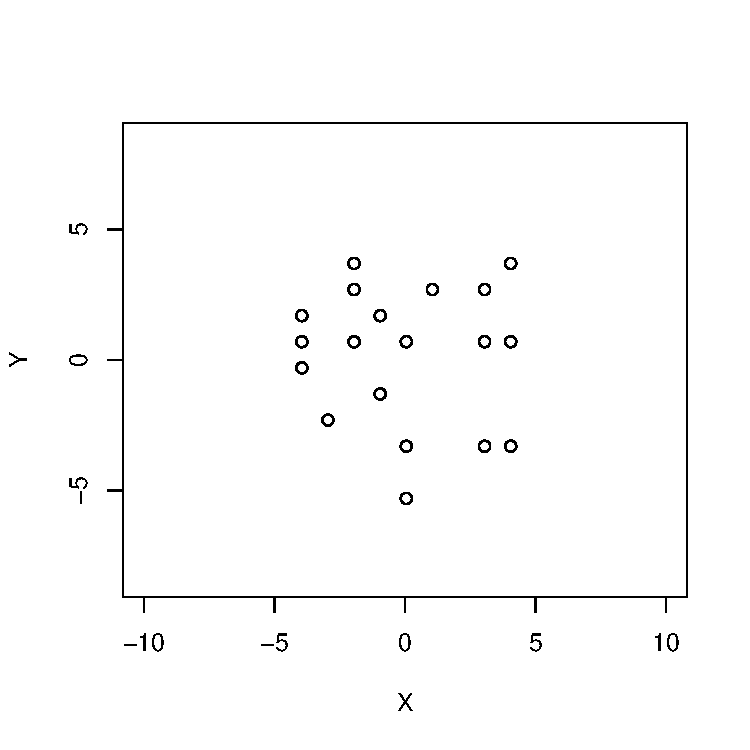
\includegraphics{ACP2print-001}
\end{frame}

\begin{frame}
\frametitle{Interpretació geomètrica}
{\small A continuació mostram les dues \red{components principals.} O sigui, les direccions on les projeccions de les 
dades tenen màxima variabilitat:}
\vspace*{-1cm}

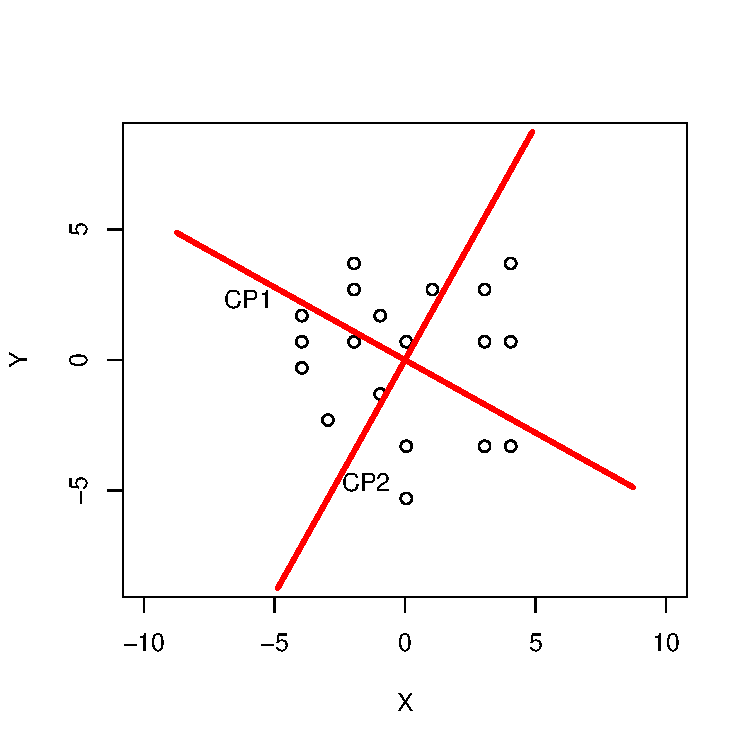
\includegraphics{ACP2print-002}
\end{frame}

\begin{frame}
\frametitle{Interpretació geomètrica}
{\small Si projectam en la direcció de la \red{primera component}, obtendrem les projeccions següents (punts blaus):}
\vspace*{-1cm}

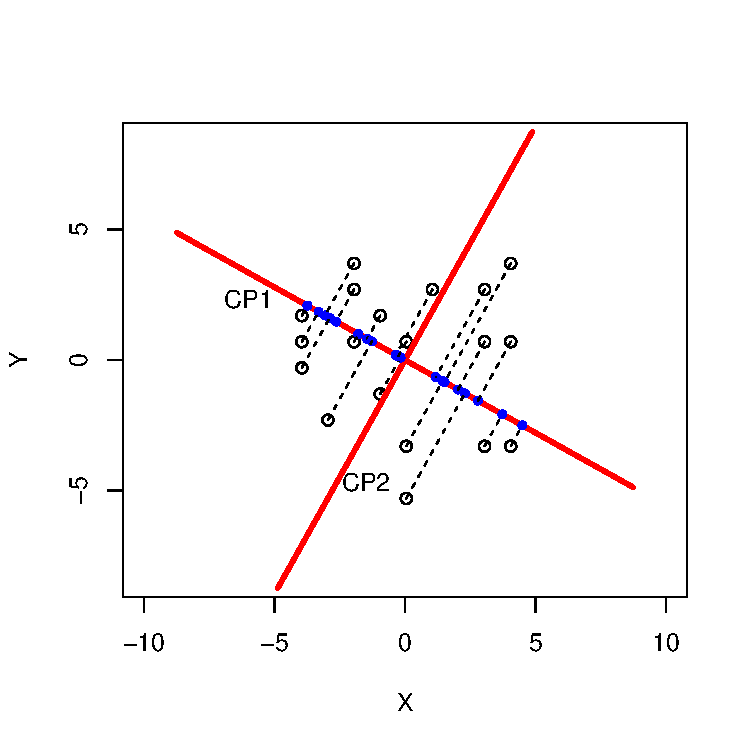
\includegraphics{ACP2print-003}
\end{frame}

\begin{frame}
\frametitle{Interpretació geomètrica}
Això significa que la variància dels punts blaus és màxima en el sentit de que si haguéssim escollit una altra direcció 
o una altra recta i haguéssim projectat sobre aquesta segona recta, la variància de les projeccions hagués estar menor.
\medskip

Els punts blaus representen les coordenades que tenen els punts de la nostra taula de dades si haguéssim agafat com eix 
d'abscisses, l'eix de la \red{primera component} $CP_1$.
\end{frame}

\begin{frame}
\frametitle{Interpretació geomètrica}
{\small Si projectam en la direcció de la \red{segona component}, obtendrem les projeccions següents (punts verds):}
\vspace*{-1cm}

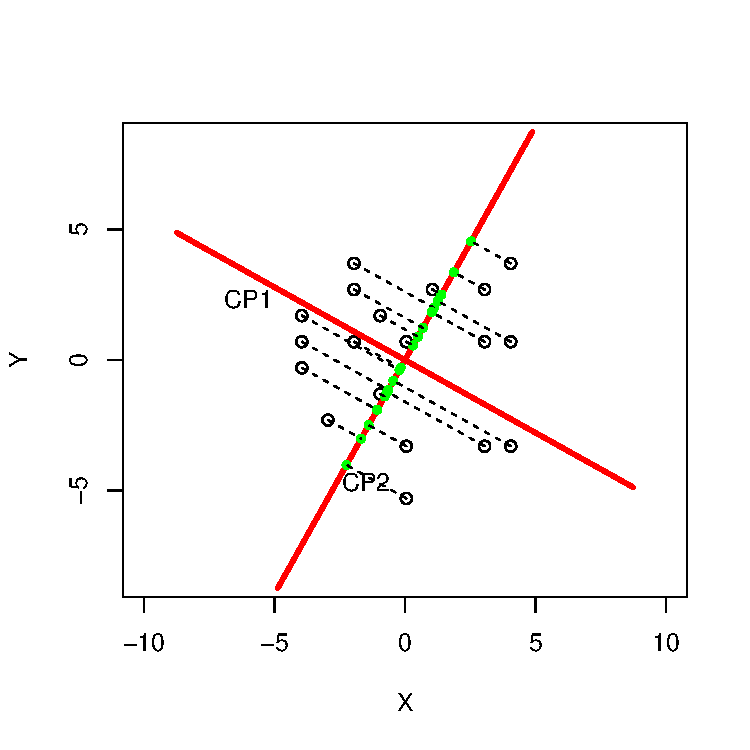
\includegraphics{ACP2print-004}
\end{frame}


\begin{frame}
\frametitle{Components principals}
Condicions han de verificar les components principals:
\begin{block}{Han d'esser incorrelades.}
O sigui, $r_{CP_i,CP_j}=0$ o si $\mathbf{y}_i$ i $\mathbf{y_j}$ són les columnes $i$ i $j$ de la matriu $\mathbf{Y}$, 
$r_{\mathbf{y}_i,\mathbf{y}_j}=0$. Dit en altres paraules, la matriu de covariàncies o de correlacions de la taula de 
dades $\mathbf{Y}$ serà diagonal.
\end{block}
\end{frame}

\begin{frame}
\frametitle{Components principals}
Condicions han de verificar les components principals:
\begin{block}{Les variàncies de les \red{components principals} han de decréixer.}
O sigui, \[
\mbox{var}(CP_1)\geq \mbox{var}(CP_2)\cdots \geq \mbox{var}(CP_p).
\]
D'aquesta forma, la \red{component principal} $CP_1$ serà la que tengui més variabilitat de totes i per tant, la més 
important, $CP_2$, la segona més important i així successivament.
\end{block}
\end{frame}


\iffalse
\begin{frame}
\frametitle{Components principals}
Condicions han de verificar les components principals:
\begin{block}{Conservació de la variabilitat}
Si $r=p$ o si tenim tantes \red{components principals} com \blue{variables originals}, la \red{variabilitat} de les 
variables s'ha de conservar:
\[
\mbox{var}(X_1)+\cdots +\mbox{var}(X_p)=\mbox{var}(CP_1)+\cdots + \mbox{var}(CP_p),
\]
o escrit en funció de les matrius $\mathbf{X}$ i $\mathbf{Y}$,
\[
s_{x_1}^2+\cdots +s_{x_p}^2 = s_{y_1}^2+\cdots + s_{y_p}^2,
\]
on $s_{x_i}^2$ és la variància de la columna $i$-èssima de la matriu~$\mathbf{X}$ i $s_{y_i^2}$ és la variància de la 
columna $i$-èssima de la matriu~$\mathbf{Y}.$
\end{block}
\end{frame}
\fi 

\iffalse
\section{Tipus d'Anàlisi de Components Principals}

\begin{frame}
\frametitle{Tipus d'Anàlisi de Components Principals}
Depenent de com sigui la matriu de dades de les \blue{originals} tenim dos tipus d'anàlisi de components principals:
\begin{itemize}
\item Si la matriu de dades $\mathbf{X}$ és centrada, l'\red{anàlisi de components principals} es diu anàlisi de 
components principals (ACP) sobre la \red{matriu de covariàncies} ja que farem servir aquesta matriu per realitzar 
l'anàlisi.
\item Si la matriu de dades $\mathbf{X}$ és tipificada, o sigui, les seves columnes, a més de tenim mitjana zero, tenen 
variància~$1$, l'\red{anàlisi de components principals} es diu anàlisi de components principals sobre la \red{matriu de 
correlacions} ja que  farem servir aquesta matriu per realitzar l'anàlisi.
\end{itemize}
\end{frame}
\fi

\section{ACP sobre la matriu de covariàncies}

\begin{frame}
\frametitle{ACP sobre la \red{matriu de covariàncies}}
Considerem $\mathbf{X}$ $n\times p$ la nostre matriu de dades que suposarem centrada on tenim $n$ individus i $p$ 
variables. Si no ho fos, l'haurem de centrar.
\bigskip

Sigui $\mathbf{S}$ $p\times p$ la matriu de covariàncies de $\mathbf{X}$.
\medskip

Recordem que $\mathbf{S}$ es calcula com:
\[
\mathbf{S}=\frac{1}{n}\mathbf{X}^\top\cdot\mathbf{X}.
\]

\end{frame}

\begin{frame}
\frametitle{ACP sobre la \red{matriu de covariàncies}}
Siguin $\lambda_1 \geq \lambda_2 \geq \cdots \geq \lambda_p$ els valors propis de la matriu~$\mathbf{S}$ en ordre 
creixent.
\medskip

Siguin $\mathbf{v}_1,\mathbf{v}_2,\ldots,\mathbf{v}_p$ els corresponents vectors propis que suposarem ortogonals i 
normalitzats. Això és, suposarem que són perpendiculars dos a dos i tenen norma euclídea unitat.
\medskip

Sigui $\mathbf{V}$ la matriu de vectors propis que té els vectors anteriors per columnes.
\medskip

Aleshores la matriu $\Lambda$ és la transposada de la matriu~$\mathbf{V}$: 
\[
\Lambda=\mathbf{V}^\top.
\]
\end{frame}

\begin{frame}[fragile]
\frametitle{ACP sobre la \red{matriu de covariàncies}}
\begin{exemple}
Considerem la següent matriu de dades:
\[
\mathbf{X}= 
\left(
% latex table generated in R 3.1.2 by xtable 1.7-4 package
% Sat Oct 24 13:16:05 2015
\begin{tabular}{rrr}
  1 & -1 & 3 \\ 
  1 & 0 & 3 \\ 
  2 & 3 & 0 \\ 
  3 & 0 & 1 \\ 
  \end{tabular}\right)
\]

\end{exemple}
\end{frame}

\begin{frame}
\frametitle{ACP sobre la \red{matriu de covariàncies}}
\begin{exemple}
Com que la matriu no està centrada, primer la centram:
{\footnotesize
\begin{eqnarray*}
\tilde{\mathbf{X}}& = & \mathbf{H}_4\mathbf{X} \\ &=&
\left(
% latex table generated in R 3.1.2 by xtable 1.7-4 package
% Sat Oct 24 13:16:05 2015
\begin{tabular}{rrrr}
  0.75 & -0.25 & -0.25 & -0.25 \\ 
  -0.25 & 0.75 & -0.25 & -0.25 \\ 
  -0.25 & -0.25 & 0.75 & -0.25 \\ 
  -0.25 & -0.25 & -0.25 & 0.75 \\ 
  \end{tabular}\right)\cdot
\left(
% latex table generated in R 3.1.2 by xtable 1.7-4 package
% Sat Oct 24 13:16:05 2015
\begin{tabular}{rrr}
  1 & -1 & 3 \\ 
  1 & 0 & 3 \\ 
  2 & 3 & 0 \\ 
  3 & 0 & 1 \\ 
  \end{tabular}\right) \\ &=&
\left(
% latex table generated in R 3.1.2 by xtable 1.7-4 package
% Sat Oct 24 13:16:05 2015
\begin{tabular}{rrr}
  -0.750 & -1.500 & 1.250 \\ 
  -0.750 & -0.500 & 1.250 \\ 
  0.250 & 2.500 & -1.750 \\ 
  1.250 & -0.500 & -0.750 \\ 
  \end{tabular}\right)
\end{eqnarray*}
}
\end{exemple}
\end{frame}

\begin{frame}
\frametitle{ACP sobre la \red{matriu de covariàncies}}
\begin{exemple}
{
La matriu de covariàncies serà:
\[
\mathbf{S}=\frac{1}{4}\tilde{\mathbf{X}}^\top\tilde{\mathbf{X}}=
\left(
% latex table generated in R 3.1.2 by xtable 1.7-4 package
% Sat Oct 24 13:16:06 2015
\begin{tabular}{rrr}
  0.688 & 0.375 & -0.812 \\ 
  0.375 & 2.250 & -1.625 \\ 
  -0.812 & -1.625 & 1.688 \\ 
  \end{tabular}\right)
\]
Els valors propis de la matriu de covariàncies anterior són:
\[
% latex table generated in R 3.1.2 by xtable 1.7-4 package
% Sat Oct 24 13:16:06 2015
\begin{tabular}{rrr}
  3.830 & 0.774 & 0.021 \\ 
  \end{tabular}\]
}
\end{exemple}
\end{frame}


\begin{frame}
\frametitle{ACP sobre la \red{matriu de covariàncies}}
\begin{exemple}
Els corresponents vectors propis (per columnes) associats als vectors propis anteriors són:
\[
% latex table generated in R 3.1.2 by xtable 1.7-4 package
% Sat Oct 24 13:16:06 2015
\begin{tabular}{rrr}
  -0.253 & 0.750 & 0.612 \\ 
  -0.722 & -0.567 & 0.396 \\ 
  0.644 & -0.342 & 0.685 \\ 
  \end{tabular}\]
Ens adonem que els vectors anteriors són ortogonals i estan normalitzats.


\end{exemple}
\end{frame}

\begin{frame}
\frametitle{ACP sobre la \red{matriu de covariàncies}}
\begin{exemple}
{\small
Així la matriu que ens canviarà de \blue{variables originals} a \red{components principals} serà la transposada dels 
vectors propis:
\[
\Lambda=
\left(
% latex table generated in R 3.1.2 by xtable 1.7-4 package
% Sat Oct 24 13:16:06 2015
\begin{tabular}{rrr}
  -0.253 & -0.722 & 0.644 \\ 
  0.750 & -0.567 & -0.342 \\ 
  0.612 & 0.396 & 0.685 \\ 
  \end{tabular}\right)
\]
Per tant, la matriu de dades en les noves variables serà:
\[
\mathbf{Y}=\tilde{\mathbf{X}}\Lambda^\top = \tilde{\mathbf{X}}\mathbf{V}=
\left(
% latex table generated in R 3.1.2 by xtable 1.7-4 package
% Sat Oct 24 13:16:06 2015
\begin{tabular}{rrr}
  2.078 & -0.139 & -0.197 \\ 
  1.355 & -0.706 & 0.199 \\ 
  -2.996 & -0.632 & -0.055 \\ 
  -0.438 & 1.477 & 0.053 \\ 
  \end{tabular}\right)
\]
}
\end{exemple}
\end{frame}

\begin{frame}
\frametitle{ACP sobre la \red{matriu de covariàncies}}
\begin{exemple}
Si calculam la matriu de covariàncies de les \red{components principals} val:
\[
\mathbf{S}_{CP}=\left(
% latex table generated in R 3.1.2 by xtable 1.7-4 package
% Sat Oct 24 13:16:06 2015
\begin{tabular}{rrr}
  3.830 & 0.000 & -0.000 \\ 
  0.000 & 0.774 & 0.000 \\ 
  -0.000 & 0.000 & 0.021 \\ 
  \end{tabular}\right)
\]
Ens adonam que és diagonal, per tant, les covariàncies entre variables diferents són nul·les i en la diagonal hi ha les 
variàncies de les \red{components principals} que estan en ordre creixent. Us sonen aquests valors?
\end{exemple}
\end{frame}

\begin{frame}
\frametitle{ACP sobre la \red{matriu de covariàncies}}
\begin{exemple}
Efectivament, són els valors propis de la matriu de covariàncies de les \blue{variables originals}~$\mathbf{S}$.
\bigskip

Comprovem que la variabilitat s'ha conservat. 
\medskip

La variabilitat de les \blue{variables originals} serà la suma dels valors de la diagonal de la matriu~$\mathbf{S}$:
\[
0.688 + 2.25 + 1.688 = 
4.625.
\]
\end{exemple}
\end{frame}


\begin{frame}
\frametitle{ACP sobre la \red{matriu de covariàncies}}
\begin{exemple}
La variabilitat de les \red{components principals} serà la suma dels valors de la diagonal de la 
matriu~$\mathbf{S}_{CP}$:
\[
3.83 + 0.774 + 0.021 = 
4.625.
\]
Podem observar que les dues variabilitats coincideixen.
\medskip

La primera \red{component principal} (1a. columna de la matriu $\mathbf{CP}$) hereta el 
$\frac{3.83}{4.625}\cdot 100\% = 
82.801\%$ de la variabilitat total.

Les dues primeres \red{components principals} hereten el 
$\frac{3.83 + 0.774}{4.625}\cdot 
100\% = 
99.544\%$ de la variabilitat total.
\end{exemple}
\end{frame}

\begin{frame}
\frametitle{ACP sobre la \red{matriu de covariàncies}}
\begin{exemple}
Facem un exemple més complet.
La taula següent ens dóna l'edat en dies ($x_1$), l'alçada al néixer en cm. ($x_2$), el seu pes en kg. en néixer ($x_3$) 
i l'augment en tant per cent del seu pes actual respecte el seu pes en néixer ($x_4$) de $9$ nens i nenes recent nats. 
\end{exemple}
\end{frame}

\begin{frame}
\frametitle{ACP sobre la \red{matriu de covariàncies}}
\begin{exemple}
{\small 
\begin{center}\begin{tabular}{|c|c|c|c|c|}\hline
$x_1$ & $x_2$ & $x_3$ & $x_4$&Sexe\\\hline
78&48.2&2.75&29.5&Nina\\ 69&45.5&2.15&26.3&Nina\\
77&46.3&4.41&32.2&Nina\\ 88&49&5.52&36.5&Nin\\ 67&43&3.21&27.2&Nina\\
80&48&4.32&27.7&Nina\\ 74&48&2.31&28.3&Nina\\ 94&53&4.3&30.3&Nin\\
102&58&3.71&28.7&Nin
\\\hline\end{tabular}\end{center}
Hem afegit una variable més (sexe de l'infant). Ens demanem si aquestes $4$ variables són capaces d'explicar o de predir 
la variable anterior. 
}
\end{exemple}
\end{frame}

\begin{frame}
\frametitle{ACP sobre la \red{matriu de covariàncies}}
\begin{exemple}
La matriu de dades centrada seria:
\[
\tilde{\mathbf{X}}=\left(
% latex table generated in R 3.1.2 by xtable 1.7-4 package
% Sat Oct 24 13:16:06 2015
\begin{tabular}{rrrr}
  -3.000 & -0.578 & -0.881 & -0.056 \\ 
  -12.000 & -3.278 & -1.481 & -3.256 \\ 
  -4.000 & -2.478 & 0.779 & 2.644 \\ 
  7.000 & 0.222 & 1.889 & 6.944 \\ 
  -14.000 & -5.778 & -0.421 & -2.356 \\ 
  -1.000 & -0.778 & 0.689 & -1.856 \\ 
  -7.000 & -0.778 & -1.321 & -1.256 \\ 
  13.000 & 4.222 & 0.669 & 0.744 \\ 
  21.000 & 9.222 & 0.079 & -1.556 \\ 
  \end{tabular}\right)
\]


\end{exemple}
\end{frame}

\begin{frame}
\frametitle{ACP sobre la \red{matriu de covariàncies}}
\begin{exemple}

La matriu de covariàncies serà:
{\small\[
\mathbf{S}=\frac{1}{9}\tilde{\mathbf{X}}^\top\tilde{\mathbf{X}}=
\left(
% latex table generated in R 3.1.2 by xtable 1.7-4 package
% Sat Oct 24 13:16:06 2015
\begin{tabular}{rrrr}
  119.333 & 43.133 & 6.148 & 10.878 \\ 
  43.133 & 17.193 & 1.148 & 1.169 \\ 
  6.148 & 1.148 & 1.111 & 2.422 \\ 
  10.878 & 1.169 & 2.422 & 8.818 \\ 
  \end{tabular}\right)
\]}
Els valors propis de la matriu de covariàncies anterior són:
\[
% latex table generated in R 3.1.2 by xtable 1.7-4 package
% Sat Oct 24 13:16:06 2015
\begin{tabular}{rrrr}
  136.296 & 9.390 & 0.722 & 0.047 \\ 
  \end{tabular}\]

\end{exemple}
\end{frame}


\begin{frame}
\frametitle{ACP sobre la \red{matriu de covariàncies}}
\begin{exemple}
Els corresponents vectors propis (per columnes) associats als vectors propis anteriors són:
\[
% latex table generated in R 3.1.2 by xtable 1.7-4 package
% Sat Oct 24 13:16:06 2015
\begin{tabular}{rrrr}
  0.935 & -0.031 & 0.250 & 0.248 \\ 
  0.340 & 0.342 & -0.665 & -0.571 \\ 
  0.047 & -0.241 & 0.572 & -0.782 \\ 
  0.084 & -0.908 & -0.411 & -0.016 \\ 
  \end{tabular}\]
Ens adonem que els vectors anteriors són ortogonals i estan normalitzats.


\end{exemple}
\end{frame}

\begin{frame}
\frametitle{ACP sobre la \red{matriu de covariàncies}}
\begin{exemple}
{
Així la matriu que ens canviarà de \blue{variables originals} a \red{components principals} serà la transposada dels 
vectors propis:
\[
\Lambda=
\left(
% latex table generated in R 3.1.2 by xtable 1.7-4 package
% Sat Oct 24 13:16:06 2015
\begin{tabular}{rrrr}
  0.935 & 0.340 & 0.047 & 0.084 \\ 
  -0.031 & 0.342 & -0.241 & -0.908 \\ 
  0.250 & -0.665 & 0.572 & -0.411 \\ 
  0.248 & -0.571 & -0.782 & -0.016 \\ 
  \end{tabular}\right)
\]
}
\end{exemple}
\end{frame}


\begin{frame}
\frametitle{ACP sobre la \red{matriu de covariàncies}}
\begin{exemple}
Les expressions de les \red{components principals} en funció de les \blue{variables originals} són:
\begin{eqnarray*}
CP_1 &=& 0.935X_1 
+0.34X_2
+0.047X_3 
+0.084X_4
\\
CP_2 &=& -0.031X_1
+0.342X_2
-0.241X_3 
-0.908X_4
\\
CP_3 &=& 0.25X_1
-0.665X_2
+0.572X_3 
-0.411X_4 \\
CP_4 &=& 0.248X_1
-0.571X_2
-0.782X_3 
-0.016X_4
\end{eqnarray*}
\end{exemple}
\end{frame}

\begin{frame}
\frametitle{ACP sobre la \red{matriu de covariàncies}}
\begin{exemple}
{\small
Per tant, la matriu de dades en les noves variables serà:
\[
\mathbf{Y}=\tilde{\mathbf{X}}\Lambda^\top = \tilde{\mathbf{X}}\mathbf{V}=
\left(
% latex table generated in R 3.1.2 by xtable 1.7-4 package
% Sat Oct 24 13:16:06 2015
\begin{tabular}{rrrr}
  -3.049 & 0.158 & -0.846 & 0.276 \\ 
  -12.683 & 2.562 & -0.328 & 0.103 \\ 
  -4.326 & -3.312 & 0.008 & -0.229 \\ 
  7.295 & -6.899 & -0.171 & 0.024 \\ 
  -15.279 & 0.696 & 1.071 & 0.190 \\ 
  -1.323 & 1.283 & 1.423 & -0.314 \\ 
  -6.980 & 1.408 & -1.471 & -0.240 \\ 
  13.691 & 0.206 & 0.517 & 0.281 \\ 
  22.655 & 3.898 & -0.202 & -0.090 \\ 
  \end{tabular}\right)
\]
}
\end{exemple}
\end{frame}

\begin{frame}
\frametitle{ACP sobre la \red{matriu de covariàncies}}
\begin{exemple}
Si calculam la matriu de covariàncies de les \red{components principals} val:
\[
\mathbf{S}_{CP}=\left(
% latex table generated in R 3.1.2 by xtable 1.7-4 package
% Sat Oct 24 13:16:06 2015
\begin{tabular}{rrrr}
  136.296 & -0.000 & 0.000 & 0.000 \\ 
  -0.000 & 9.390 & -0.000 & -0.000 \\ 
  0.000 & -0.000 & 0.722 & 0.000 \\ 
  0.000 & -0.000 & 0.000 & 0.047 \\ 
  \end{tabular}\right)
\]
Igual que passava en l'exemple anterior, és diagonal, com esperàvem i en la diagonal hi surten els valors propis de la 
matriu de covariàncies de les \blue{dades originals.}
\end{exemple}
\end{frame}


\begin{frame}
\frametitle{ACP sobre la \red{matriu de covariàncies}}
\begin{exemple}
Comprovem que la variabilitat s'ha conservat. 
\medskip

La variabilitat de les \blue{variables originals} serà la suma dels valors de la diagonal de la matriu~$\mathbf{S}$:
\[
119.333 + 17.193 + 
1.111 + 8.818 = 146.455.
\]
La variabilitat de les \red{components principals} serà la suma dels valors de la diagonal de la 
matriu~$\mathbf{S}_{CP}$:
\[
136.296 + 9.39 + 0.722 
+0.047= 146.455.
\]
Podem observar que les dues variabilitats coincideixen.
\end{exemple}
\end{frame}

\begin{frame}
\frametitle{ACP sobre la \red{matriu de covariàncies}}
\begin{exemple}

La primera \red{component principal} (1a. columna de la matriu $\mathbf{CP}$) hereta el 
$\frac{136.296}{146.455}\cdot 100\% = 
93.064\%$ de la variabilitat total.

Les dues primeres \red{components principals} hereten el 
$\frac{136.296 + 
9.39}{146.455}\cdot 100\% = 
99.475\%$ de la variabilitat total.
\end{exemple}
\end{frame}

\begin{frame}
\frametitle{ACP sobre la \red{matriu de covariàncies}}
\begin{exemple}
Això ens fa pensar que si només tenim en compte les dues primeres components, podem fer un gràfic on hi estiguin 
representats tots els nens dibuixant de blau els nens i de vermell les nenes.
\medskip

Comprovem que les dues primeres components separen bé els nens i les nens. Concloem que la nostra taula de dades 
``explica'' la variable sexe.
\end{exemple}
\end{frame}

\begin{frame}
\frametitle{ACP sobre la \red{matriu de covariàncies}}
\begin{exemple}
\vspace*{-1cm}

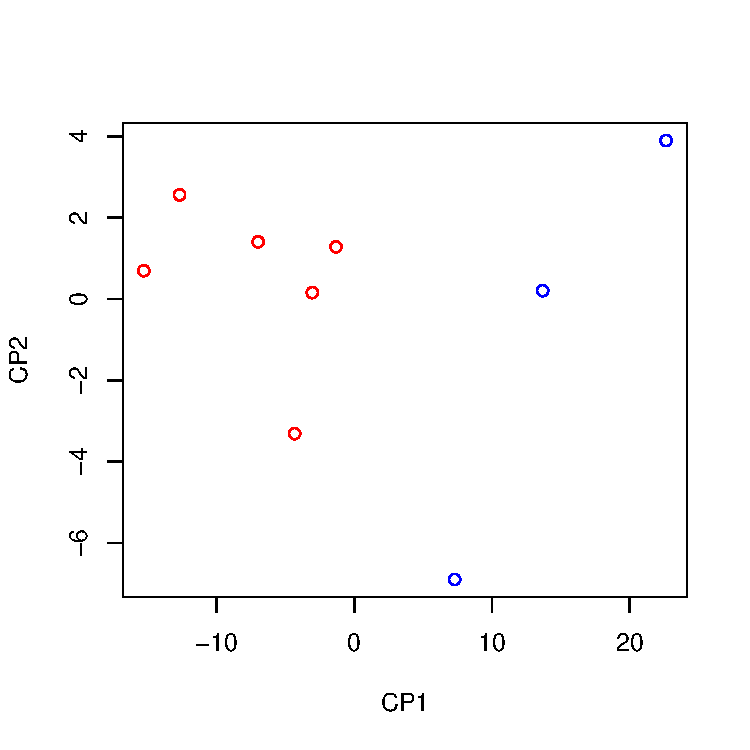
\includegraphics{ACP2print-030}
\end{exemple}
\end{frame}

\section{Propietats de l'ACP sobre la matriu de covariàncies}
\begin{frame}
\frametitle{Propietats de l'ACP sobre la \red{matriu de covariàncies}}
Recordem que la matriu $\mathbf{S}$ és la matriu de covariàncies de les \blue{variables originals} i $\mathbf{S}_{CP}$ 
és la matriu de covariàncies de les \red{components principals.}
\medskip

La diagonal de la matriu $\mathbf{S}$ està formada per les variàncies de les \blue{variables originals} $s_i^2$, 
$i=1,\ldots,p$.
\medskip

Definim la \red{variància total} de la nostra taula de dades com la suma de les variàncies o la traça de la 
matriu~$\mathbf{S}$:
\[
\mbox{Variància Total}=tr(\mathbf{S})=\sum_{i=1}^p s_i^2.
\]
\end{frame}


\begin{frame}
\frametitle{Propietats de l'ACP sobre la \red{matriu de covariàncies}}
\begin{itemize}
\item La variància de la $i$-èssima \red{component principal} és el \red{valor propi} $i$-èssim de la matriu de 
covariàncies~$\mathbf{S}$: $\mbox{Var} (CP)_i =\lambda_i.$
\item Es conserva la variància total. O sigui, la variància total de les \blue{variables originals} i de les 
\red{components principals} és la mateixa:
\[
\sum_{i=1}^p \mbox{var}(X_i) = \sum_{i=1}^p \mbox{var}(CP_i) =\sum_{i=1}^p\lambda_i.
\]

\end{itemize}
\end{frame}

\begin{frame}
\frametitle{Propietats de l'ACP sobre la \red{matriu de covariàncies}}
\begin{itemize}
\item Les \red{components principals} són incorrelades. O, dit, en altres paraules, la seva matriu de covariàncies és 
diagonal:
$$\mathbf{S}_{CP}=\left(\begin{array}{cccc}
\lambda_1& 0 &\ldots &  0\\
0& \lambda_{2}&\ldots & 0\\
\vdots & \vdots & & \vdots\\
0 & 0&\ldots &  \lambda_{p}
\end{array}
\right)$$

\end{itemize}
\end{frame}


\begin{frame}
\frametitle{Propietats de l'ACP sobre la \red{matriu de covariàncies}}
{\small
\begin{itemize}
\item Donada una taula de dades, definim la \red{variància generalitzada} com el determinant de la matriu de 
covariàncies. Aleshores, la \red{variància generalitzada} de les \blue{variables originals} i de les \red{components 
principals} coincideix:
\[
\mbox{det}(\mathbf{S}) =\mbox{det}(\mathbf{S}_{CP}) =\lambda_1\cdots \lambda_p.
\]
\item La proporció de variància explicada per la \red{component $j$-èssima} és: 
$\frac{\lambda_j}{\sum_{i=1}^p\lambda_i}.$ Per tant, la variància explicada per les \red{$k$ primeres components} val: 
$\frac{\sum_{i=1}^k\lambda_j}{\sum_{i=1}^p\lambda_i}.$

\end{itemize}
}
\end{frame}


\begin{frame}
\frametitle{Propietats de l'ACP sobre la \red{matriu de covariàncies}}
{\small
\begin{itemize}
\item Sigui $\mathbf{X}_i$ la $i$-èssima \blue{variable original}. O sigui, la $i$-èssima columna de la matriu de 
dades~$\mathbf{X}$. Sigui $\mathbf{CP}_j$ la \red{$j$-èssima component principal}. O sigui, la $j$-èssima columna de la 
matriu de dades~$\mathbf{CP}$. Aleshores la covariància entre les variables (columnes) $\mathbf{X}_i$ i $\mathbf{CP}_j$ 
val:
\[
\mbox{cov}(\mathbf{X}_i,\mathbf{CP}_j)=\lambda_j u_{ji},
\]
on $u_{ji}$ és la $i$-èssima component del vector propi unitari $\mathbf{u}_j$ corresponent al valor propi~$\lambda_j.$ 

\item Seguin la mateixa notació anterior, la correlació entre $\mathbf{X}_i$ i $\mathbf{CP}_j$ val:
\[
\mbox{cor}(\mathbf{X}_i,\mathbf{CP}_j)=\frac{\sqrt{\lambda_j}u_{ji}}{s_i}.
\]
\end{itemize}
}
\end{frame}

\begin{frame}
\frametitle{Propietats de l'ACP sobre la \red{matriu de covariàncies}}
\begin{itemize}
\item En general si definim la matriu $\mathbf{S}_{X,CP}$ de components $s_{ij}=\mbox{cov}(\mathbf{X}_i,\mathbf{CP}_j)$, 
podem escriure:
\[
\mathbf{S}_{X,CP}= \mathbf{V}\mbox{diag}(\lambda_1,\ldots,\lambda_p),
\]
on $\mathbf{V}$ és la matriu de vectors propis de la matriu de covariàncies~$\mathbf{S}.$
\item En general si definim la matriu $\mathbf{R}_{X,CP}$ de components $r_{ij}=\mbox{cor}(\mathbf{X}_i,\mathbf{CP}_j)$, 
podem escriure:
\[
\mathbf{R}_{X,CP}= 
\mathbf{V}\mbox{diag}(\sqrt{\lambda_1},\ldots,\sqrt{\lambda_p})\mbox{diag}\left(\frac{1}{s_1},\ldots,\frac{1}{s_p}
\right),
\]
on $s_i$ és la desviació típica de la \blue{variable original} $\mathbf{X}_i$.
\end{itemize}
\end{frame}

\begin{frame}
\frametitle{Propietats de l'ACP sobre la \red{matriu de covariàncies}}
La primera \red{component principal} seria la varietat lineal de dimensió~$1$ (una recta) que conserva la major 
\red{variabilitat} (anomenada \red{inèrcia}) del ``núvol'' de punts.
\medskip

De la mateixa manera, les dues primeres \red{components principals} serien la varietat lineal de dimensió~$2$ (pla) que 
conserva la major \red{variabilitat} (anomenada \red{inèrcia}) del ``núvol'' de punts.
\medskip

En general, les $k$ primeres \red{components principals} serien la varietat lineal de dimensió~$k$ que conserva la major 
\red{variabilitat} (anomenada \red{inèrcia}) del ``núvol'' de punts.


\end{frame}


\begin{frame}
\frametitle{Exemple}
\begin{exemple}
Comprovem la relació anterior entre les \blue{variables originals} i les \red{components principals} en l'exemple dels 
infants.
Recordem que la matriu centrada de dades era:
\[
\tilde{\mathbf{X}}=\left(
% latex table generated in R 3.1.2 by xtable 1.7-4 package
% Sat Oct 24 13:16:06 2015
\begin{tabular}{rrrr}
  -3.0 & -0.6 & -0.9 & -0.1 \\ 
  -12.0 & -3.3 & -1.5 & -3.3 \\ 
  -4.0 & -2.5 & 0.8 & 2.6 \\ 
  7.0 & 0.2 & 1.9 & 6.9 \\ 
  -14.0 & -5.8 & -0.4 & -2.4 \\ 
  -1.0 & -0.8 & 0.7 & -1.9 \\ 
  -7.0 & -0.8 & -1.3 & -1.3 \\ 
  13.0 & 4.2 & 0.7 & 0.7 \\ 
  21.0 & 9.2 & 0.1 & -1.6 \\ 
  \end{tabular}\right)
\]
\end{exemple}
\end{frame}

\begin{frame}
\frametitle{Exemple}
\begin{exemple}
La matriu de \red{components principals} era:
\[
{\mathbf{CP}}=\left(
% latex table generated in R 3.1.2 by xtable 1.7-4 package
% Sat Oct 24 13:16:06 2015
\begin{tabular}{rrrr}
  -3.049 & 0.158 & -0.846 & 0.276 \\ 
  -12.683 & 2.562 & -0.328 & 0.103 \\ 
  -4.326 & -3.312 & 0.008 & -0.229 \\ 
  7.295 & -6.899 & -0.171 & 0.024 \\ 
  -15.279 & 0.696 & 1.071 & 0.190 \\ 
  -1.323 & 1.283 & 1.423 & -0.314 \\ 
  -6.980 & 1.408 & -1.471 & -0.240 \\ 
  13.691 & 0.206 & 0.517 & 0.281 \\ 
  22.655 & 3.898 & -0.202 & -0.090 \\ 
  \end{tabular}\right)
\]
\end{exemple}
\end{frame}


\begin{frame}
\frametitle{Exemple}
\begin{exemple}
La covariància entre les dues matrius anteriors val:
\[
\mbox{cov}(\tilde{X},{\mathbf{CP}})=\left(
% latex table generated in R 3.1.2 by xtable 1.7-4 package
% Sat Oct 24 13:16:06 2015
\begin{tabular}{rrrr}
  127.503 & -0.289 & 0.180 & 0.012 \\ 
  46.349 & 3.210 & -0.480 & -0.027 \\ 
  6.397 & -2.263 & 0.413 & -0.036 \\ 
  11.426 & -8.524 & -0.296 & -0.001 \\ 
  \end{tabular}\right)
\]

\end{exemple}
\end{frame}


\begin{frame}
\frametitle{Exemple}
\begin{exemple}
Si fem $\mathbf{V}\mbox{diag}(\lambda_1,\ldots,\lambda_p)$ obtenim el mateix:
{
\begin{eqnarray*}
&&\left(
% latex table generated in R 3.1.2 by xtable 1.7-4 package
% Sat Oct 24 13:16:06 2015
\begin{tabular}{rrrr}
  0.935 & -0.031 & 0.250 & 0.248 \\ 
  0.340 & 0.342 & -0.665 & -0.571 \\ 
  0.047 & -0.241 & 0.572 & -0.782 \\ 
  0.084 & -0.908 & -0.411 & -0.016 \\ 
  \end{tabular}\right)\cdot
\\ && \hspace*{1cm}\left(
% latex table generated in R 3.1.2 by xtable 1.7-4 package
% Sat Oct 24 13:16:06 2015
\begin{tabular}{rrrr}
  136.296 & 0.000 & 0.000 & 0.000 \\ 
  0.000 & 9.390 & 0.000 & 0.000 \\ 
  0.000 & 0.000 & 0.722 & 0.000 \\ 
  0.000 & 0.000 & 0.000 & 0.047 \\ 
  \end{tabular}\right) \\ && = \mbox{cov}(\tilde{X},{\mathbf{CP}})
\end{eqnarray*}

}

\end{exemple}
\end{frame}


\begin{frame}
\frametitle{Exemple}
\begin{exemple}
La correlacions entre les dues matrius anteriors val:
\[
\mbox{cor}(\tilde{X},{\mathbf{CP}})=\left(
% latex table generated in R 3.1.2 by xtable 1.7-4 package
% Sat Oct 24 13:16:06 2015
\begin{tabular}{rrrr}
  1.000 & -0.009 & 0.019 & 0.005 \\ 
  0.957 & 0.253 & -0.136 & -0.030 \\ 
  0.520 & -0.701 & 0.461 & -0.160 \\ 
  0.330 & -0.937 & -0.118 & -0.001 \\ 
  \end{tabular}\right)
\]

\end{exemple}
\end{frame}

\begin{frame}
\frametitle{Exemple}
\begin{exemple}
Si fem 
$\mathbf{V}\mbox{diag}(\sqrt{\lambda_1},\ldots,\sqrt{\lambda_p})\mbox{diag}\left(\frac{1}{s_1},\ldots,\frac{1}{s_p}
\right)$ obtenim el mateix, o sigui el producte de les tres matrius següents:
\begin{eqnarray*}
\mathbf{V} &=&\left(
% latex table generated in R 3.1.2 by xtable 1.7-4 package
% Sat Oct 24 13:16:06 2015
\begin{tabular}{rrrr}
  0.935 & -0.031 & 0.250 & 0.248 \\ 
  0.340 & 0.342 & -0.665 & -0.571 \\ 
  0.047 & -0.241 & 0.572 & -0.782 \\ 
  0.084 & -0.908 & -0.411 & -0.016 \\ 
  \end{tabular}\right)\\
\mbox{diag}(\sqrt{\lambda}) &=&\left(
% latex table generated in R 3.1.2 by xtable 1.7-4 package
% Sat Oct 24 13:16:06 2015
\begin{tabular}{rrrr}
  11.675 & 0.000 & 0.000 & 0.000 \\ 
  0.000 & 3.064 & 0.000 & 0.000 \\ 
  0.000 & 0.000 & 0.850 & 0.000 \\ 
  0.000 & 0.000 & 0.000 & 0.216 \\ 
  \end{tabular}\right)
\end{eqnarray*}


\end{exemple}
\end{frame}

\begin{frame}
\frametitle{Exemple}
\begin{exemple}
\[
\mbox{diag}(1/s)=\left(
% latex table generated in R 3.1.2 by xtable 1.7-4 package
% Sat Oct 24 13:16:06 2015
\begin{tabular}{rrrr}
  0.092 & 0.000 & 0.000 & 0.000 \\ 
  0.000 & 0.241 & 0.000 & 0.000 \\ 
  0.000 & 0.000 & 0.949 & 0.000 \\ 
  0.000 & 0.000 & 0.000 & 0.337 \\ 
  \end{tabular}\right)
\]

\end{exemple}
\end{frame}

\begin{frame}
\frametitle{Exemple}
\begin{exemple}
Vegem quin percentatge de variabilitat tenim si consideram només les primeres \red{components principals}:
\begin{center}
\begin{tabular}{|l|l|}\hline
Variables&Varianza Explicada\\\hline
$\mathbf{CP}_1$&$136.296/146.455=
0.931$\\\hline
$\mathbf{CP}_{1,2}$&$145.686/146.455=
0.995$\\\hline
$\mathbf{CP}_{1,2,3}$&$146.408/146.455=
0.9997$\\\hline
$\mathbf{CP}_{1,2,3,4}$&$1$\\\hline
\end{tabular}
\end{center}
En aquest exemple, si només tenguéssim en compte les dues \red{primeres components} explicaríem el 
$99.48\%$ de la \red{variabilitat} total.

\end{exemple}
\end{frame}

\section{ACP sobre la matriu de correlacions}
\begin{frame}
\frametitle{ACP sobre la \red{matriu de correlacions}}
Per realitzar l'ACP sobre la matriu de correlacions, es fa de la mateixa manera que l'ACP sobre la matriu de 
covariàncies però en lloc de fer servir aquesta matriu es fa servir la matriu de correlacions~$\mathbf{R}.$
\medskip

O sigui, es calculen els valors propis $\lambda_i$ de la matriu~$\mathbf{R}$ juntament amb la matriu de vectors 
propis~$\mathbf{V}$.
\medskip

Això és equivalent a aplicar l'ACP sobre la matriu de covariàncies però en lloc de fer servir la matriu centrada 
original, es fa servir la matriu de dades tipificada~$\mathbf{Z}.$
\medskip

Per tant, totes les propietats enunciades sobre la \red{matriu de covariàncies} serien vàlides per la \red{matriu de 
correlacions} substituint simplement la matriu $\mathbf{S}$ per la matriu $\mathbf{R}.$
\end{frame}

\begin{frame}
\frametitle{ACP sobre la \red{matriu de correlacions}}
\begin{exemple}
Anem a repetir l'exemple dels infants però fent una ACP sobre la \red{matriu de correlacions.}

Recordem les dades:
{\small 
\begin{center}\begin{tabular}{|c|c|c|c|c|}\hline
$x_1$ & $x_2$ & $x_3$ & $x_4$&Sexe\\\hline
78&48.2&2.75&29.5&Nina\\ 69&45.5&2.15&26.3&Nina\\
77&46.3&4.41&32.2&Nina\\ 88&49&5.52&36.5&Nin\\ 67&43&3.21&27.2&Nina\\
80&48&4.32&27.7&Nina\\ 74&48&2.31&28.3&Nina\\ 94&53&4.3&30.3&Nin\\
102&58&3.71&28.7&Nin
\\\hline\end{tabular}\end{center}
}
\end{exemple}
\end{frame}

\begin{frame}
\frametitle{ACP sobre la \red{matriu de correlacions}}
La matriu de dades tipificada serà:
\[
{\mathbf{R}}=\left(
% latex table generated in R 3.1.2 by xtable 1.7-4 package
% Sat Oct 24 13:16:06 2015
\begin{tabular}{rrrr}
  -0.275 & -0.139 & -0.836 & -0.019 \\ 
  -1.099 & -0.791 & -1.405 & -1.096 \\ 
  -0.366 & -0.598 & 0.739 & 0.891 \\ 
  0.641 & 0.054 & 1.792 & 2.339 \\ 
  -1.282 & -1.393 & -0.400 & -0.793 \\ 
  -0.092 & -0.188 & 0.654 & -0.625 \\ 
  -0.641 & -0.188 & -1.254 & -0.423 \\ 
  1.190 & 1.018 & 0.635 & 0.251 \\ 
  1.922 & 2.224 & 0.075 & -0.524 \\ 
  \end{tabular}\right)
\]
\end{frame}







\begin{frame}
\frametitle{ACP sobre la \red{matriu de correlacions}}
\begin{exemple}
La matriu de correlacions~$\mathbf{R}$ de la matriu $\mathbf{X}$ o la matriu de covariàncies de la matriu~$\mathbf{Z}$ 
serà:
\[
{\mathbf{R}}=\left(
% latex table generated in R 3.1.2 by xtable 1.7-4 package
% Sat Oct 24 13:16:06 2015
\begin{tabular}{rrrr}
  1.000 & 0.952 & 0.534 & 0.335 \\ 
  0.952 & 1.000 & 0.263 & 0.095 \\ 
  0.534 & 0.263 & 1.000 & 0.774 \\ 
  0.335 & 0.095 & 0.774 & 1.000 \\ 
  \end{tabular}\right)
\]
Els valors propis de la matriu de correlacions anterior són:
\[
% latex table generated in R 3.1.2 by xtable 1.7-4 package
% Sat Oct 24 13:16:06 2015
\begin{tabular}{rrrr}
  2.503 & 1.286 & 0.208 & 0.003 \\ 
  \end{tabular}\]

\end{exemple}
\end{frame}


\begin{frame}
\frametitle{ACP sobre la \red{matriu de correlacions}}
\begin{exemple}
Els corresponents vectors propis (per columnes) associats als vectors propis anteriors són:
\[
% latex table generated in R 3.1.2 by xtable 1.7-4 package
% Sat Oct 24 13:16:06 2015
\begin{tabular}{rrrr}
  -0.579 & 0.352 & -0.014 & 0.735 \\ 
  -0.482 & 0.566 & 0.171 & -0.647 \\ 
  -0.506 & -0.444 & -0.712 & -0.199 \\ 
  -0.420 & -0.599 & 0.681 & -0.031 \\ 
  \end{tabular}\]
Ens adonem que els vectors anteriors són ortogonals i estan normalitzats.


\end{exemple}
\end{frame}

\begin{frame}
\frametitle{ACP sobre la \red{matriu de correlacions}}
\begin{exemple}
{
Així la matriu que ens canviarà de \blue{variables originals} a \red{components principals} serà la transposada dels 
vectors propis:
\[
\Lambda=
\left(
% latex table generated in R 3.1.2 by xtable 1.7-4 package
% Sat Oct 24 13:16:06 2015
\begin{tabular}{rrrr}
  -0.579 & -0.482 & -0.506 & -0.420 \\ 
  0.352 & 0.566 & -0.444 & -0.599 \\ 
  -0.014 & 0.171 & -0.712 & 0.681 \\ 
  0.735 & -0.647 & -0.199 & -0.031 \\ 
  \end{tabular}\right)
\]
}
\end{exemple}
\end{frame}


\begin{frame}
\frametitle{ACP sobre la \red{matriu de correlacions}}
\begin{exemple}
Les expressions de les \red{components principals} en funció de les \blue{variables originals} tipificades són:
\begin{eqnarray*}
CP_1 &=& -0.579Z_1 
-0.482Z_2
-0.506Z_3 
-0.42Z_4
\\
CP_2 &=& 0.352Z_1
+0.566Z_2
-0.444Z_3 
-0.599Z_4
\\
CP_3 &=& -0.014Z_1
+0.171Z_2
-0.712Z_3 
+0.681Z_4 \\
CP_4 &=& 0.735Z_1
-0.647Z_2
-0.199Z_3 
-0.031Z_4
\end{eqnarray*}
\end{exemple}
\end{frame}

\begin{frame}
\frametitle{ACP sobre la \red{matriu de correlacions}}
\begin{exemple}
{\small
Per tant, la matriu de dades en les noves variables serà:
\[
\mathbf{Y}={\mathbf{Z}}\Lambda^\top = {\mathbf{Z}}\mathbf{V}=
\left(
% latex table generated in R 3.1.2 by xtable 1.7-4 package
% Sat Oct 24 13:16:06 2015
\begin{tabular}{rrrr}
  0.657 & 0.207 & 0.563 & 0.056 \\ 
  2.189 & 0.446 & 0.134 & 0.018 \\ 
  -0.249 & -1.329 & -0.017 & -0.058 \\ 
  -2.287 & -1.941 & 0.316 & 0.007 \\ 
  1.949 & -0.587 & -0.476 & 0.063 \\ 
  0.075 & -0.054 & -0.922 & -0.057 \\ 
  1.274 & 0.478 & 0.582 & -0.087 \\ 
  -1.606 & 0.563 & -0.124 & 0.082 \\ 
  -2.002 & 2.216 & -0.056 & -0.024 \\ 
  \end{tabular}\right)
\]
}
\end{exemple}
\end{frame}

\begin{frame}
\frametitle{ACP sobre la \red{matriu de correlacions}}
\begin{exemple}
Si calculam la matriu de correlacions de les \red{components principals} val:
\[
\mathbf{R}_{CP}=\left(
% latex table generated in R 3.1.2 by xtable 1.7-4 package
% Sat Oct 24 13:16:06 2015
\begin{tabular}{rrrr}
  1.000 & 0.000 & 0.000 & -0.000 \\ 
  0.000 & 1.000 & 0.000 & -0.000 \\ 
  0.000 & 0.000 & 1.000 & 0.000 \\ 
  -0.000 & -0.000 & 0.000 & 1.000 \\ 
  \end{tabular}\right)
\]
Surt la matriu diagonal, fet que posa de manifest que les \red{components principals} són incorrelades.
\end{exemple}
\end{frame}



\begin{frame}
\frametitle{ACP sobre la \red{matriu de correlacions}}
\begin{exemple}

La primera \red{component principal} (1a. columna de la matriu $\mathbf{CP}$) hereta el 
$\frac{2.503}{4}\cdot 100\% = 
62.575\%$ de la variabilitat total.

Les dues primeres \red{components principals} hereten el 
$\frac{2.503 + 1.286}{4}\cdot 100\% = 
94.732\%$ de la variabilitat total.
\end{exemple}
\end{frame}

\begin{frame}
\frametitle{ACP sobre la \red{matriu de correlacions}}
\begin{exemple}
Això ens fa pensar que si només tenim en compte les dues primeres components, podem fer un gràfic on hi estiguin 
representats tots els nens dibuixant de blau els nens i de vermell les nenes.
\medskip

Comprovem que les dues primeres components separen bé els nens i les nens. Concloem que la nostra taula de dades 
``explica'' la variable sexe.
\end{exemple}
\end{frame}

\begin{frame}
\frametitle{ACP sobre la \red{matriu de correlacions}}
\begin{exemple}
\vspace*{-1cm}

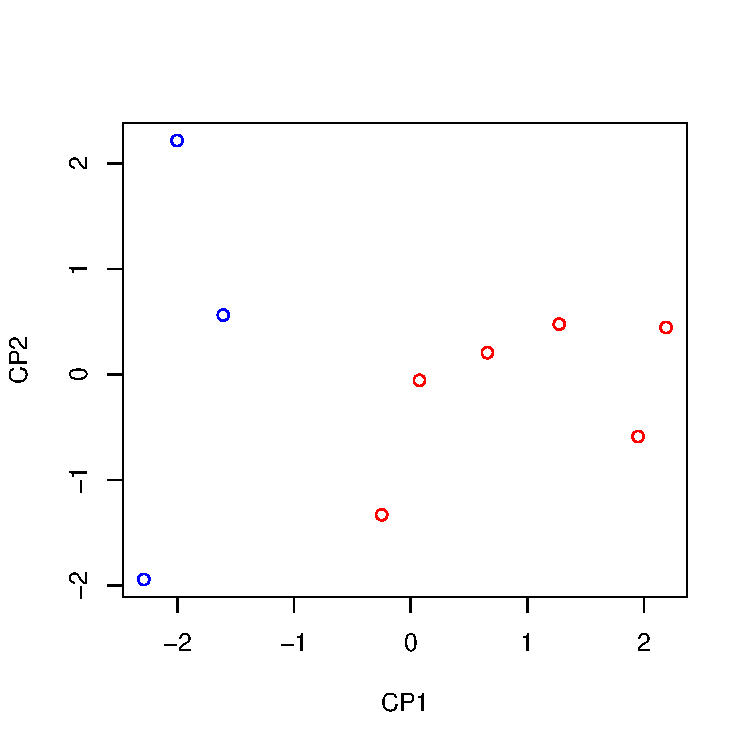
\includegraphics{ACP2print-051}
\end{exemple}
\end{frame}

\section{Etapes d'un ACP}

\begin{frame}
\frametitle{Etapes d'un ACP}
\begin{itemize}
\item \blue{Primera etapa:} decidir si es realitza l'ACP damunt les dades brutes centrades (matriu de covariàncies) o 
sobre les dades tipificades (matriu de correlacions).
\begin{itemize}
\item Quan les variables originals $\mathbf{X}$ estan en unitats distintes, convé aplicar l'\red{ACP de correlacions}. 
Si estan en les mateixes unitats, ambdues alternatives són vàlides.
\item Si les diferències entre les variàncies són informatives i volem tenir-les en compte en l'anàlisi, no hem 
d'estandaritzar les variables i aplicar l'\red{ACP de covariàncies}.
\end{itemize}
\end{itemize}
\end{frame}


\begin{frame}
\frametitle{Etapes d'un ACP}
\begin{itemize}
\item \blue{Segona etapa:} reducció de la dimensionalitat. Hem de decidir quantes components retenim. La quantitat de 
variància retenguda serà:
\begin{center}
\begin{tabular}{|c|c|c|}\hline
Comp. & Valor propi & Quantitat retinguda\\\hline
$Cp_1$  & $\lambda_1$ & $\lambda_1/\sum_{i=1}^p \lambda_i$\\
$Cp_2 $ & $\lambda_2$ & $(\lambda_1+\lambda_2)/\sum_{i=1}^p \lambda_i$\\
$Cp_3$ & $\lambda_3$ &
$(\lambda_1+\lambda_2+\lambda_3)/\sum_{i=1}^p
\lambda_i$\\ $\ldots$ & $\ldots$ & $\ldots$\\
$Cp_p$ & $\lambda_p$ &
$(\lambda_1+\ldots+\lambda_p)/\sum_{i=1}^p \lambda_i=1$\\\hline
\end{tabular}
\end{center}
\end{itemize}
\end{frame}


\begin{frame}
\frametitle{Etapes d'un ACP}
\begin{itemize}
\item \blue{Segona etapa:} Per decidir el  nombre de components retingudes, hi ha dos mètodes:
\begin{itemize}
\item Seleccionar components fins cobrir una proporció determinada de variància, com el $80\%$ o el $90\%$. 
\item Mètode de la mitjana aritmètica. Se retenen totes aquelles components $\mathbf{CP}_i$ que compleixin que 
$\lambda_i \geq \overline{\lambda}=\frac{\sum_{i=1}^p \lambda_i}{p}$. En el cas de l'\red{ACP de correlacions}, la 
condició anterior és $\lambda_i\geq 1$.
\end{itemize}
\end{itemize}
\end{frame}

\begin{frame}
\frametitle{Etapes d'un ACP}
\begin{exemple}
En l'exemple dels infants,
\begin{itemize}
\item si aplicam el primer mètode per decidir el nombre de components retingudes, fent l'\red{ACP de correlacions}, si 
només elegim la primera component, ja cobrim el $62.575\%$ de la variància 
total. Si elegim les dues primeres, cobrim el $94.732\%$ de la 
variància total.
\item si aplicam el mètode de la mitjana aritmètica, hauríem de retenir dues components ja que  els valors propis de la 
matriu de correlacions~$\mathbf{R}$ eren 
$
% latex table generated in R 3.1.2 by xtable 1.7-4 package
% Sat Oct 24 13:16:06 2015
\begin{tabular}{rrrr}
  2.503 & 1.286 & 0.208 & 0.003 \\ 
  \end{tabular}$.
\end{itemize}
\end{exemple}
\end{frame}


\section{Descomposició en valors singulars (SVD)}
\begin{frame}
\frametitle{Descomposició en valors singulars}
Donada una matriu de dades $\mathbf{X}$ de dimensions $n\times p$, on $n\geq p$ i de rang~$p$, es pot descompondre en 
producte de tres matrius:
\[
\mathbf{X}=\mathbf{U}\Sigma\mathbf{V}^\top,
\]
on
\begin{itemize}
\item $\mathbf{U}$ és una matriu ortogonal $n\times p$ que té per columnes els $p$ vectors propis de la matriu 
$\mathbf{X}\mathbf{X}^\top$ associats als $p$ valors propis no nuls.
\item ${\Sigma}$ és una matriu diagonal $p\times p$ que té per diagonal les arrels quadrades dels valors propis de la 
matriu $\mathbf{X}^\top\mathbf{X}$.
\item $\mathbf{V}$ és una matriu ortogonal $p\times p$ que té per columnes els vectors propis de la matriu 
$\mathbf{X}^\top\mathbf{X}$ associats als $p$ valors propis no nuls.
\end{itemize}
\end{frame}


\begin{frame}
\frametitle{Descomposició en valors singulars (SVD)}
\begin{exemple}
Considerem la matriu $\mathbf{X}$ com la matriu de dades centrada de l'exemple dels infants.
\medskip

La matriu $\mathbf{X}^\top\mathbf{X}$ val:
\[
\mathbf{X}^\top\mathbf{X}=\left(
% latex table generated in R 3.1.2 by xtable 1.7-4 package
% Sat Oct 24 13:16:06 2015
\begin{tabular}{rrrr}
  1074.000 & 388.200 & 55.330 & 97.900 \\ 
  388.200 & 154.736 & 10.330 & 10.521 \\ 
  55.330 & 10.330 & 9.995 & 21.795 \\ 
  97.900 & 10.521 & 21.795 & 79.362 \\ 
  \end{tabular}\right)
\]
\end{exemple}
\end{frame}

\begin{frame}
\frametitle{Descomposició en valors singulars (SVD)}
\begin{exemple}
La matriu $\mathbf{X}\mathbf{X}^\top$ val: (mostram només les 4 primeres columnes, pensau que és $10\times 10$)
{\footnotesize
\[
\mathbf{X}^\top\mathbf{X}=\left(
% latex table generated in R 3.1.2 by xtable 1.7-4 package
% Sat Oct 24 13:16:06 2015
\begin{tabular}{rrrr}
  10.113 & 39.380 & 12.598 & -23.179 \\ 
  39.380 & 167.536 & 46.359 & -110.134 \\ 
  12.598 & 46.359 & 29.739 & -8.715 \\ 
  -23.179 & -110.134 & -8.715 & 100.843 \\ 
  45.840 & 195.231 & 63.759 & -116.437 \\ 
  2.945 & 19.570 & 1.557 & -18.757 \\ 
  22.683 & 92.594 & 25.578 & -60.387 \\ 
  -42.070 & -173.254 & -59.972 & 98.371 \\ 
  -68.311 & -277.281 & -110.903 & 138.396 \\ 
  \end{tabular}\right)
\]
}
\end{exemple}
\end{frame}


\begin{frame}
\frametitle{Descomposició en valors singulars  (SVD)}
\begin{exemple}
Els valors propis de la matriu $\mathbf{X}^\top\mathbf{X}$ són:
\[
% latex table generated in R 3.1.2 by xtable 1.7-4 package
% Sat Oct 24 13:16:06 2015
\begin{tabular}{rrrr}
  1226.665 & 84.511 & 6.498 & 0.419 \\ 
  \end{tabular}\]
Per tant, la matriu $\Sigma$ serà:
\[
\Sigma =\left(
% latex table generated in R 3.1.2 by xtable 1.7-4 package
% Sat Oct 24 13:16:06 2015
\begin{tabular}{rrrr}
  35.024 & 0.000 & 0.000 & 0.000 \\ 
  0.000 & 9.193 & 0.000 & 0.000 \\ 
  0.000 & 0.000 & 2.549 & 0.000 \\ 
  0.000 & 0.000 & 0.000 & 0.647 \\ 
  \end{tabular}\right)
\]
\end{exemple}
\end{frame}


\begin{frame}
\frametitle{Descomposició en valors singulars (SVD)}
\begin{exemple}
La matriu $\mathbf{U}$ serà la següent matriu $10\times 4$:
\[
\mathbf{U} =\left(
% latex table generated in R 3.1.2 by xtable 1.7-4 package
% Sat Oct 24 13:16:06 2015
\begin{tabular}{rrrr}
  -0.087 & 0.017 & 0.332 & 0.426 \\ 
  -0.362 & 0.279 & 0.129 & 0.159 \\ 
  -0.124 & -0.360 & -0.003 & -0.354 \\ 
  0.208 & -0.750 & 0.067 & 0.037 \\ 
  -0.436 & 0.076 & -0.420 & 0.294 \\ 
  -0.038 & 0.140 & -0.558 & -0.485 \\ 
  -0.199 & 0.153 & 0.577 & -0.371 \\ 
  0.391 & 0.022 & -0.203 & 0.434 \\ 
  0.647 & 0.424 & 0.079 & -0.140 \\ 
  \end{tabular}\right)
\]
\end{exemple}
\end{frame}


\begin{frame}
\frametitle{Descomposició en valors singulars (SVD)}
\begin{exemple}
La matriu $\mathbf{V}$ serà la següent matriu $4\times 4$:
\[
\mathbf{U} =\left(
% latex table generated in R 3.1.2 by xtable 1.7-4 package
% Sat Oct 24 13:16:06 2015
\begin{tabular}{rrrr}
  0.935 & -0.031 & -0.250 & 0.248 \\ 
  0.340 & 0.342 & 0.665 & -0.571 \\ 
  0.047 & -0.241 & -0.572 & -0.782 \\ 
  0.084 & -0.908 & 0.411 & -0.016 \\ 
  \end{tabular}\right)
\]

Es pot comprovar que $\mathbf{X}=\mathbf{U}\Sigma\mathbf{V}^\top$.
\end{exemple}
\end{frame}

\section{Relació  ACP amb SVD}

\begin{frame}
\frametitle{Relació ACP amb SVD}
Considerem una matriu de dades $\mathbf{X}$ $n\times p$ que pot ésser centrada (\red{ACP de covariàncies}) o tipificada 
(\red{ACP de correlacions}).
\medskip

Si considerem la seva \red{SVD}, $\mathbf{X}=\mathbf{U}\Sigma\mathbf{V}^\top$, tenim que les \red{components 
principals}, $\mathbf{Y}$, valen $\mathbf{CP}=\mathbf{U}\Sigma$.
\medskip

{\footnotesize
La prova és molt senzilla. Recordem que les components principals valien: $\mathbf{CP}=\mathbf{X}\mathbf{V}$, on 
$\mathbf{V}$ era la matriu de vectors propis de la matriu de covariàncies 
$\mathbf{S}=\frac{1}{n}\mathbf{X}^\top\mathbf{X}$. Ara bé, aquesta matriu coincidirà amb la matriu de vectors propis de 
la matriu $\mathbf{X}^\top\mathbf{X}$ ja que els vectors propis de la matriu anterior i de la matriu de covariàncies 
$\mathbf{S}$ són els mateixos.

Per tant, 
$$\mathbf{Y}=\mathbf{X}\mathbf{V}=\mathbf{U}\Sigma\mathbf{V}^\top\mathbf{V}=\mathbf{U}\Sigma,$$
ja que la matriu $\mathbf{V}$ és ortogonal.}
\end{frame}

\begin{frame}
\frametitle{Relació ACP amb SVD}
\begin{teorema}
El producte escalar de dues \blue{files} de la matriu de dades $\mathbf{X}$ coincideix amb el producte escalar de dues 
\blue{files} de la matriu de  \red{components principals} $\mathbf{Y}$.
\end{teorema}
{\footnotesize
Prova. El producte escalar de dues files de la matriu~$\mathbf{X}$ ve donada per la matriu $\mathbf{X}\mathbf{X}^\top$ 
però:
\[
\mathbf{X}\mathbf{X}^\top = \mathbf{Y}\mathbf{V}^\top\mathbf{V}\mathbf{Y}^\top =\mathbf{Y}\mathbf{Y}^\top,
\]
aquesta última matriu ens dóna el producte escalar de dues files de la matriu de \red{components principals.}
}
\end{frame}

\begin{frame}
\frametitle{Relació ACP amb SVD}
\begin{teorema}
La distància euclídea de dues files de la matriu $\mathbf{X}$ coincideix amb la distància euclídea de la matriu de 
\red{components principals} $\mathbf{Y}$. O sigui, la distància entre els individus respecte les \blue{variables 
originals} i respecte les \red{components principals} se conserva.
\end{teorema}
{\footnotesize Prova. Siguin $\mathbf{f}_i$ i $\mathbf{f}_j$ dues files de la matriu $\mathbf{X}$ i siguin 
$\mathbf{g}_i$ i $\mathbf{g}_j$ dues files de la matriu $\mathbf{Y}$. Aleshores:
\[
\|\mathbf{f}_i-\mathbf{f}_j\|^2 = (\mathbf{f}_i-\mathbf{f}_j)^\top 
(\mathbf{f}_i-\mathbf{f}_j)=\mathbf{f}_i^\top\mathbf{f}_i-2\mathbf{f}_i^\top\mathbf{f}_j+\mathbf{f}_j^\top\mathbf{f}_j.
\]
Ara bé, fent servir el teorema anterior tenim que:
\[
\mathbf{f}_i^\top\mathbf{f}_i=\mathbf{g}_i^\top\mathbf{g}_i,\ 
\mathbf{f}_i^\top\mathbf{f}_j=\mathbf{g}_i^\top\mathbf{g}_j, \ 
\mathbf{f}_j^\top\mathbf{f}_j=\mathbf{g}_j^\top\mathbf{g}_j.
\]
Concloem, doncs:
\(
\|\mathbf{f}_i-\mathbf{f}_j\|^2=\|\mathbf{g}_i-\mathbf{g}_j\|^2.
\)
}
\end{frame}


\begin{frame}
\frametitle{Relació ACP amb SVD}
\begin{teorema}
Sigui $\mathbf{X}$ la nostra matriu de dades originals centrada o tipificada. Sigui 
$\mathbf{X}=\mathbf{U}\Sigma\mathbf{V}^\top$ la seva \red{SVD}. Considerem la matriu $\mathbf{V}_2 = 
\Sigma\mathbf{V}^\top$. Aleshores el producte escalar de dues \blue{columnes} de la matriu $\mathbf{X}$ i de dues 
\blue{columnes} de la matriu $\mathbf{V}_2$ és el mateix.
\end{teorema}
{\footnotesize Prova.
El producte escalar de dues columnes de la matriu $\mathbf{X}$ ho dóna la matriu $\mathbf{X}^\top\mathbf{X}$. Tendrem:
\[
\mathbf{X}^\top\mathbf{X}=\mathbf{V}\Sigma\mathbf{U}^\top\mathbf{U}\Sigma\mathbf{V}^\top = \mathbf{V}\Sigma 
(\mathbf{V}\Sigma)^\top = \mathbf{V}_2^\top\mathbf{V}_2,
\]
matriu que dóna el producte escalar de dues columnes de la matriu~$\mathbf{V}_2$.
}
\end{frame}


\begin{frame}
\frametitle{Relació ACP amb SVD}
\begin{teorema}
Sigui $\mathbf{X}$ la nostra matriu de dades originals centrada o tipificada. Sigui 
$\mathbf{X}=\mathbf{U}\Sigma\mathbf{V}^\top$ la seva \red{SVD}. Considerem la matriu $\mathbf{V}_2 = 
\Sigma\mathbf{V}^\top$. Aleshores la correlació entre dues columnes de la matriu $\mathbf{X}$ i la correlació entre dues 
columnes de la matriu $\mathbf{V}_2 = \Sigma\mathbf{V}^\top$ és la mateixa.
O sigui, la correlació entre dues \blue{variables originals} (dues columnes de la matriu~$\mathbf{X}$) i dues columnes 
de la matriu $\mathbf{V}_2$ és la mateixa.
\end{teorema}

Per la prova, basta aplicar el teorema anterior. 
\end{frame}

\section{Biplots}
\begin{frame}
\frametitle{Biplots}
Per representar el resultat d'un ACP gràficament es fa servir el que s'anomena un \red{biplot}. 
\medskip

Un \red{biplot} és un gràfic bidimensional on es representa en el mateix gràfic els individus i les \blue{variables 
originals.}
\medskip

El \red{biplot} només té significat si la variabilitat explicada per les dues primeres \red{components principals} és 
alta, posem d'un $85\%$ o més. 
\medskip

En un \red{biplot} hi ha $4$ eixos coordenats: dos fan referència als individus (eixos d'abaix i de l'esquerra) i dos 
fan referència a les \blue{variables originals.} (eixos de dalt i de la dreta)
\end{frame}

\begin{frame}
\frametitle{Biplots}
Els eixos que fan referència als individus són els corresponents a les dues \red{components principals}.
\medskip

Per tant, les coordenades dels individus seran els valors de les dues \red{primeres components} estandaritzades (ja 
veurem què significa això amb un exemple).
\medskip

Hem vist que la distància euclídea entre els valors originals dels individus (files de la matriu de dades~$\mathbf{X}$) 
i els valors d'aquests mateixos individus respecte les \red{components principals} se conserva. Això significa que si 
les dues primeres \red{components principals} expliquen molta variabilitat, la distància entre individus que es veurà al 
\red{biplot} serà aproximadament la distància entre els individus segons les \blue{variables originals.}
\medskip

\end{frame}


\begin{frame}
\frametitle{Biplots}

Les coordenades corresponents a les \blue{variables originals} (columnes de la matriu de dades~$\mathbf{X}$) les ens 
dóna les dues primeres components en columnes de la matriu $\mathbf{V}_2 = \Sigma\mathbf{V}^\top$ ja que hem vist que la 
correlació entre les \blue{variables originals} i les columnes de la matriu anterior és la mateixa.

\end{frame}

\begin{frame}
\frametitle{Biplots}
El gràfic de les \blue{variables originals} es va mitjançant vectors. La interpretació que s'ha de fer és la següent: si 
l'angle entre dues \blue{variables originals} és petit, significa que el cosinus d'aquest angle serà gran però aquest 
cosinus és la correlació entre les dues variables. Per tant, hi haurà molta correlació entre les variables. En canvi, si 
l'angle entre les dues variables està proper a un angle recte, la correlació entre aquestes variables és quasi nul·la.
\medskip

Les llargades dels vectors són les variàncies de les \blue{variables originals}. Per tant, com més llarg tengui un 
vector, la variable corresponent tendrà més dispersió.
\end{frame}



\begin{frame}
\frametitle{Biplots}
\begin{exemple}
Considerem l'exemple dels infants fent l'\red{ACP de covariàncies}.

Recordem que les dues primeres \red{components principals} explicaven el 
$99.475\%$ de la variabilitat total.

Les \red{components principals} eren les següents:
{\footnotesize
\[
\mathbf{Y}=
\left(
% latex table generated in R 3.1.2 by xtable 1.7-4 package
% Sat Oct 24 13:16:06 2015
\begin{tabular}{rrrr}
  -3.049 & 0.158 & -0.846 & 0.276 \\ 
  -12.683 & 2.562 & -0.328 & 0.103 \\ 
  -4.326 & -3.312 & 0.008 & -0.229 \\ 
  7.295 & -6.899 & -0.171 & 0.024 \\ 
  -15.279 & 0.696 & 1.071 & 0.190 \\ 
  -1.323 & 1.283 & 1.423 & -0.314 \\ 
  -6.980 & 1.408 & -1.471 & -0.240 \\ 
  13.691 & 0.206 & 0.517 & 0.281 \\ 
  22.655 & 3.898 & -0.202 & -0.090 \\ 
  \end{tabular}\right)
\]
}
\end{exemple}
\end{frame}


\begin{frame}
\frametitle{Biplots}
\begin{exemple}
Quan representem els individus (nens i nenes) en el \red{biplot} representarem les dues primeres columnes de la matriu 
anterior tipificada. 

Això significa que dividirem cada element de la matriu per la norma euclídea de la columna. Així la norma euclídea de la 
primera columna de la matriu anterior val:
\[
\sqrt{3.049^2+\cdots+22.655^2}=
35.024.
\]
Fent el mateix amb la segona columna,
\[
\sqrt{0.158^2+\cdots+3.898^2}=
9.193.
\]
\end{exemple}
\end{frame}


\begin{frame}
\frametitle{Biplots}
\begin{exemple}
Les coordenades dels nens i nenes en el biplot seran:
\[
\left(
% latex table generated in R 3.1.2 by xtable 1.7-4 package
% Sat Oct 24 13:16:06 2015
\begin{tabular}{rr}
  -3.049 & 0.158 \\ 
  -12.683 & 2.562 \\ 
  -4.326 & -3.312 \\ 
  7.295 & -6.899 \\ 
  -15.279 & 0.696 \\ 
  -1.323 & 1.283 \\ 
  -6.980 & 1.408 \\ 
  13.691 & 0.206 \\ 
  22.655 & 3.898 \\ 
  \end{tabular}\right)
\left(
\begin{array}{cc}
\frac{1}{35.024}&0\\
0&\frac{1}{9.193}
\end{array}
\right)=
\]
\end{exemple}
\end{frame}


\begin{frame}
\frametitle{Biplots}
\begin{exemple}
Les coordenades dels nens i nenes en el biplot seran:
\[
\left(
% latex table generated in R 3.1.2 by xtable 1.7-4 package
% Sat Oct 24 13:16:06 2015
\begin{tabular}{rr}
  -0.087 & 0.017 \\ 
  -0.362 & 0.279 \\ 
  -0.124 & -0.360 \\ 
  0.208 & -0.750 \\ 
  -0.436 & 0.076 \\ 
  -0.038 & 0.140 \\ 
  -0.199 & 0.153 \\ 
  0.391 & 0.022 \\ 
  0.647 & 0.424 \\ 
  \end{tabular}\right)
\]
\end{exemple}
\end{frame}


\begin{frame}
\frametitle{Biplots}
\begin{exemple}
Passem ara a calcular les coordenades de les \blue{variables originals}.
\medskip

Recordem que la matriu de vectors propis de la matriu de covariàncies~$\mathbf{S}$ era:
\[
\left(
% latex table generated in R 3.1.2 by xtable 1.7-4 package
% Sat Oct 24 13:16:06 2015
\begin{tabular}{rrrr}
  0.935 & -0.031 & 0.250 & 0.248 \\ 
  0.340 & 0.342 & -0.665 & -0.571 \\ 
  0.047 & -0.241 & 0.572 & -0.782 \\ 
  0.084 & -0.908 & -0.411 & -0.016 \\ 
  \end{tabular}\right)
\]
\end{exemple}
\end{frame}

\begin{frame}
\frametitle{Biplots}
\begin{exemple}
Si fem la \red{SVD} de la matriu de dades centrada $\tilde{\mathbf{X}}$, la matriu $\Sigma$ serà:
\[
\Sigma=\left(
% latex table generated in R 3.1.2 by xtable 1.7-4 package
% Sat Oct 24 13:16:06 2015
\begin{tabular}{rrrr}
  35.024 & 0.000 & 0.000 & 0.000 \\ 
  0.000 & 9.193 & 0.000 & 0.000 \\ 
  0.000 & 0.000 & 2.549 & 0.000 \\ 
  0.000 & 0.000 & 0.000 & 0.647 \\ 
  \end{tabular}\right)
\]
Per tant, la matriu $\mathbf{V}_2 =\Sigma\mathbf{V}^\top$ serà:
\[
\mathbf{V}_2 = \left(
% latex table generated in R 3.1.2 by xtable 1.7-4 package
% Sat Oct 24 13:16:06 2015
\begin{tabular}{rrrr}
  32.764 & 11.910 & 1.644 & 2.936 \\ 
  -0.283 & 3.143 & -2.216 & -8.345 \\ 
  0.636 & -1.694 & 1.459 & -1.047 \\ 
  0.161 & -0.370 & -0.507 & -0.010 \\ 
  \end{tabular}\right)
\]
\end{exemple}
\end{frame}

\begin{frame}
\frametitle{Biplots}
\begin{exemple}
Per tant, les coordenades de les $4$ variables originals són:
\begin{itemize}
\item[${\mathbf{x}_1}$]: Edat en dies. $\left(
% latex table generated in R 3.1.2 by xtable 1.7-4 package
% Sat Oct 24 13:16:06 2015
\begin{tabular}{rr}
  32.764 & -0.283 \\ 
  \end{tabular}\right)
$

\item[${\mathbf{x}_2}$]: Alçada en néixer. $\left(
% latex table generated in R 3.1.2 by xtable 1.7-4 package
% Sat Oct 24 13:16:06 2015
\begin{tabular}{rr}
  11.910 & 3.143 \\ 
  \end{tabular}\right)
$

\item[${\mathbf{x}_3}$]: Pes en néixer $\left(
% latex table generated in R 3.1.2 by xtable 1.7-4 package
% Sat Oct 24 13:16:06 2015
\begin{tabular}{rr}
  1.644 & -2.216 \\ 
  \end{tabular}\right)
$

\item[${\mathbf{x}_4}$]: Augment en tant per cent del seu pes actual respecte del seu pes en néixer $\left(
% latex table generated in R 3.1.2 by xtable 1.7-4 package
% Sat Oct 24 13:16:06 2015
\begin{tabular}{rr}
  2.936 & -8.345 \\ 
  \end{tabular}\right)
$
\end{itemize}
\end{exemple}
\end{frame}

\begin{frame}
\frametitle{Biplots}
A continuació mostram el biplot:
\vspace*{0cm}

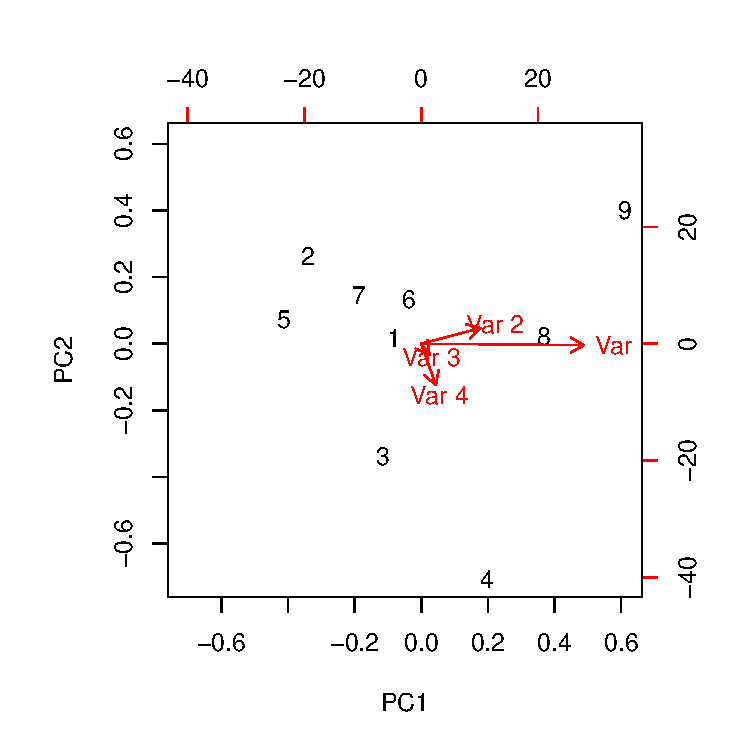
\includegraphics{ACP2print-072}
\end{frame}

\begin{frame}
\frametitle{Biplots}
Comprovem les coordenades dels punts i de les variables.
\medskip

Veiem també que entre les parelles de variables $(\mathbf{x}_1, \mathbf{x}_2)$ i   $(\mathbf{x}_3,\mathbf{x}_4)$ hi ha 
bastanta correlació i entre les parelles $(\mathbf{x}_2, \mathbf{x}_3)$ i $(\mathbf{x}_2, \mathbf{x}_4)$ n'hi ha poca 
com podem comprovar si calculem la correlació entre les variables originals:
\[
\left(
% latex table generated in R 3.1.2 by xtable 1.7-4 package
% Sat Oct 24 13:16:06 2015
\begin{tabular}{rrrr}
  1.000 & 0.952 & 0.534 & 0.335 \\ 
  0.952 & 1.000 & 0.263 & 0.095 \\ 
  0.534 & 0.263 & 1.000 & 0.774 \\ 
  0.335 & 0.095 & 0.774 & 1.000 \\ 
  \end{tabular}\right)
\]
Observem que les variables amb més dispersió són l'edat de l'infant i l'alçada en néixer.
\end{frame}

\end{document}



